\documentclass[11pt]{article}
    \title{\textbf{Maths IA - Written 8}}
    \date{}
    \usepackage{amssymb}
    \usepackage{amsmath}
    \usepackage{multirow}
    \usepackage{graphicx}
	\graphicspath{ {./} }
    \author{Jack Larkin}
    \addtolength{\topmargin}{-3cm}
    \addtolength{\textheight}{3cm}
\begin{document}
\maketitle
\section*{Algebra}
The plot of the given constraints, with feasible region shaded, is shown in Figure 1. It was generated using MATLAB.
\begin{figure}[h]
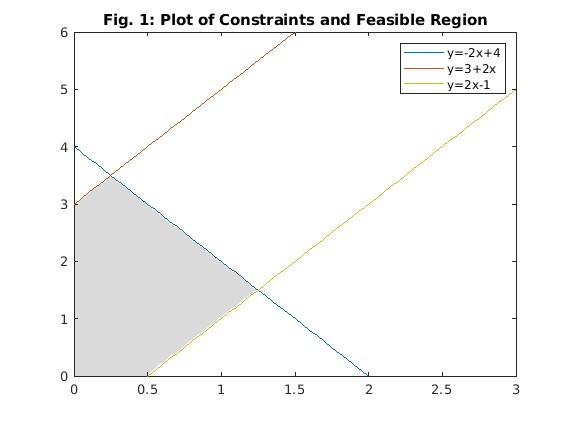
\includegraphics[scale=2.7]{plot1}
\end{figure}
\subsection*{(b)}
$$\begin{bmatrix}
2 &1 \\
-2 &y \\
2 &-1 \\
\end{bmatrix}
\begin{bmatrix}
x & y\\

\end{bmatrix}
\leq
\begin{bmatrix}
4\\
3\\
1\\
\end{bmatrix},
\begin{bmatrix}
x & y\\
\end{bmatrix}
\geq 0$$
\subsection*{(c)}
The vertices of this feasible region can be found by finding each point where constraint lines intersect, if such points exist. In this case given that $y=3+2x$ is parallel to $y=2x-1$, only the points where the $x$ or $y$ axes or $y=-2x+4$ intersects either of these lines need to be considered, leading us to the following five vertices:
\\

1. $(0,0)$\\

2. $(0,3)$\\

3. $(0.5,0)$\\

4. $(1.25,1.5)$\\

5. $(0.25,3.5)$\\

\section*{Calculus}
The first step in calculating the given integral is to split it up into an integral of $f(x)$ and an integral of $g(x)$, both with coefficients, rather than one large compound integral:
$$2\int_{-1}^{5} f(x)dx-4\int_{-1}^{5} g(x)dx$$ 
Now this can be broken further still into the pieces which comprise the piecewise functions $f(x)$ and $g(x)$ as follows: 
$$2(\int_{-1}^{2} f(x)dx+\int_{2}^{3} f(x)dx+\int_{3}^{5} f(x)dx)-4(\int_{-1}^{2} g(x)dx + \int_{2}^{4} g(x)dx)$$ 
And from here we can do away with calculus in favour of simple geometry. Armed with the knowledge that the integral of a function is equal to the area bounded by it and the x axis, and is negative when it is below the x axis, it can be deduced by observation that: 
$$\int_{-1}^{2} f(x)dx=\frac{3\times 3}{2}=4.5$$
$$\int_{2}^{3} f(x)dx=\frac{3\times 1}{2}=1.5$$
$$\int_{3}^{5} f(x)dx=\frac{-1\times 2}{2}=-1$$
And similarly that:
$$\int_{-1}^{2} g(x)dx=\pi \times 1.5^2 \times 0.5=\frac{9\pi}{8}$$
$$\int_{-1}^{2} g(x)dx=\pi \times -1 \times 0.5 =\frac{-\pi}{2}$$
SinceSo the integral can be rewritten as:
$$2(4.5+1.5-1)-4(\frac{9\pi}{8}-\frac{\pi}{2})$$
Which is much nicer on the eyes, and is equal to:
$$10-\frac{5\pi}{2}$$
\end{document}